\documentclass{article}
\usepackage[margin=1in]{geometry}
\usepackage{amsmath,amsthm,amssymb}
\usepackage{bbm,enumerate,mathtools}
\usepackage{tikz,pgfplots}
\usepackage{chessboard}
\usepackage[hidelinks]{hyperref}
\usepackage{multicol} % Problem 35

\newenvironment{question}{\begin{trivlist}\item[\textbf{Question.}]}{\end{trivlist}}
\newenvironment{note}{\begin{trivlist}\item[\textbf{Note.}]}{\end{trivlist}}
\newenvironment{references}{\begin{trivlist}\item[\textbf{References.}]}{\end{trivlist}}
\newenvironment{related}{\begin{trivlist}\item[\textbf{Related.}]\end{trivlist}\begin{enumerate}}{\end{enumerate}}


\begin{document}
\rating{2}{3}
Say that an $n$-robot takes steps that are $1/n$ of a circle ($2\pi/n$ radians).
Call a $(k, j)$-step pattern a walk that starts with $k$ right turns, followed
by $j$ left turns, followed by $k$ right turns, and so on until the robot
reaches its original position in the original orientation.
\begin{figure}[ht!]
  \centering
  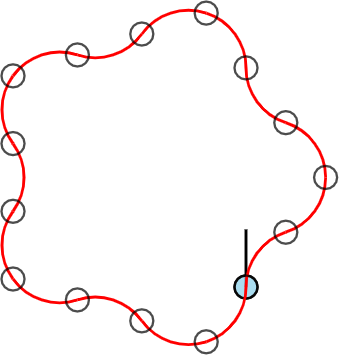
\includegraphics[scale=0.18]{assets/robot_walks/079_problem_5-robot_1_2.png}
  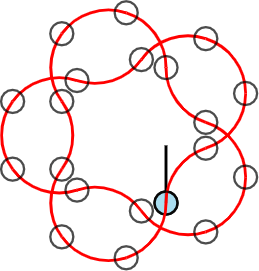
\includegraphics[scale=0.18]{assets/robot_walks/079_problem_5-robot_1_3.png}
  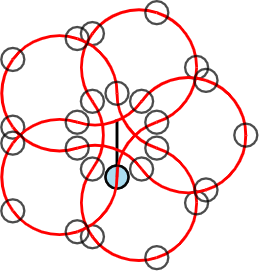
\includegraphics[scale=0.18]{assets/robot_walks/079_problem_5-robot_1_4.png}
  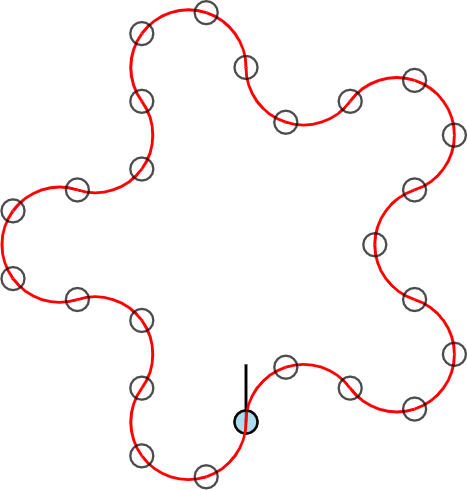
\includegraphics[scale=0.18]{assets/robot_walks/079_problem_5-robot_2_3.png}
  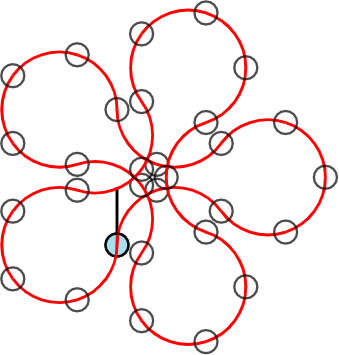
\includegraphics[scale=0.18]{assets/robot_walks/079_problem_5-robot_2_4.png}
  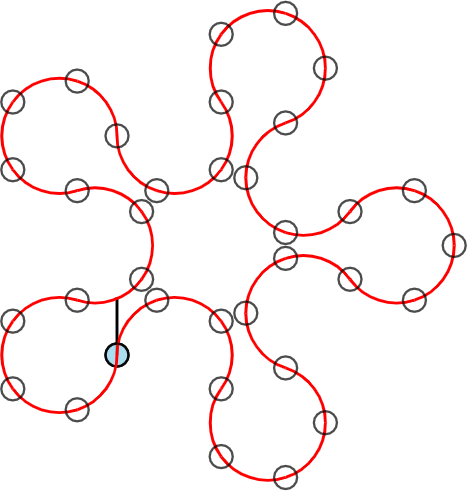
\includegraphics[scale=0.18]{assets/robot_walks/079_problem_5-robot_3_4.png}
  \caption{
    A $5$-robot walks in $(1,2)$, $(1,3)$, $(1,4)$, $(2,3)$,
    $(2,4)$, and $(3,4)$-step patterns, respectively.
  }
\end{figure}
\begin{figure}[ht!]
  \centering
  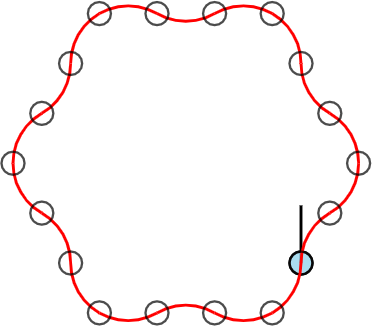
\includegraphics[scale=0.12]{assets/robot_walks/079_problem_6-robot_1_2.png}
  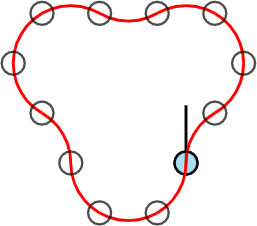
\includegraphics[scale=0.12]{assets/robot_walks/079_problem_6-robot_1_3.png}
  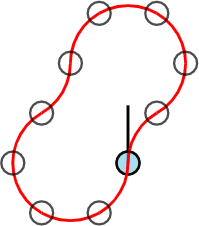
\includegraphics[scale=0.12]{assets/robot_walks/079_problem_6-robot_1_4.png}
  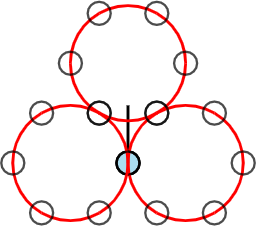
\includegraphics[scale=0.12]{assets/robot_walks/079_problem_6-robot_1_5.png}
  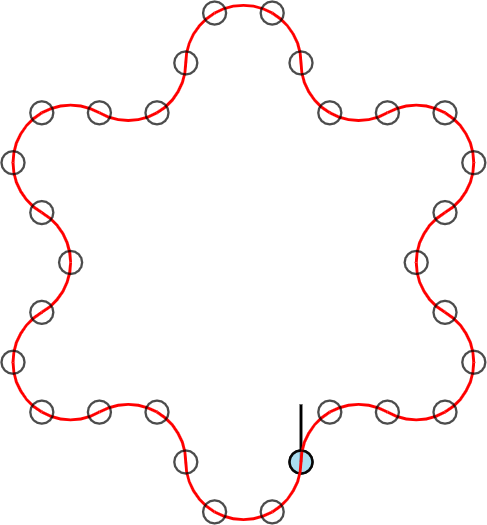
\includegraphics[scale=0.12]{assets/robot_walks/079_problem_6-robot_2_3.png}
  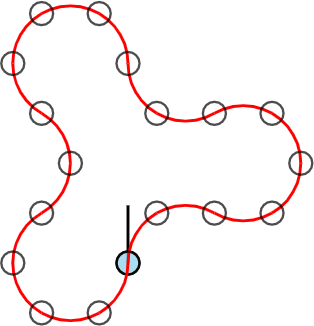
\includegraphics[scale=0.12]{assets/robot_walks/079_problem_6-robot_2_4.png}
  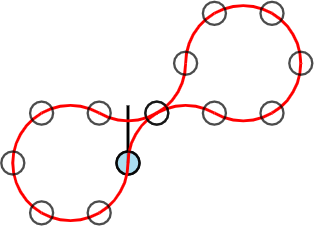
\includegraphics[scale=0.12]{assets/robot_walks/079_problem_6-robot_2_5.png}
  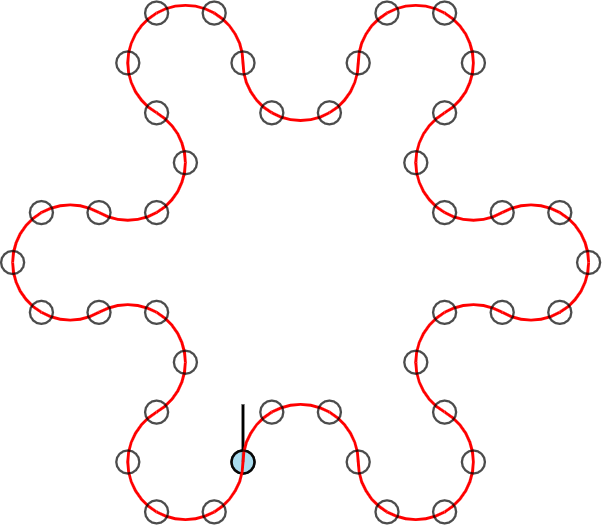
\includegraphics[scale=0.12]{assets/robot_walks/079_problem_6-robot_3_4.png}
  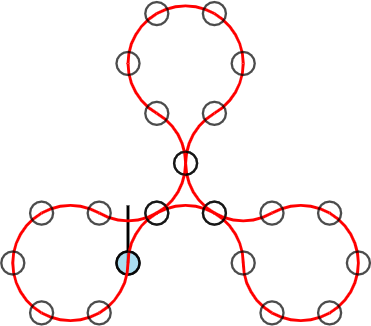
\includegraphics[scale=0.12]{assets/robot_walks/079_problem_6-robot_3_5.png}
  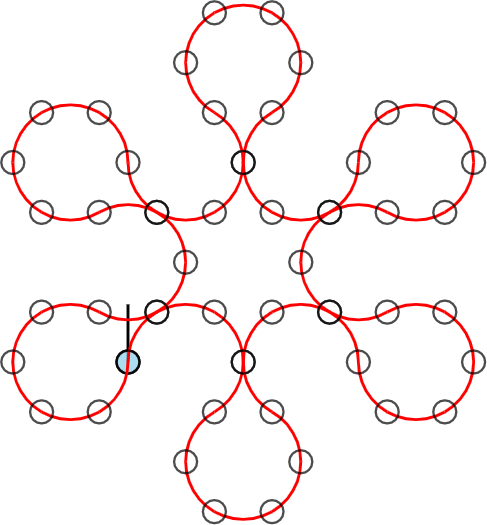
\includegraphics[scale=0.12]{assets/robot_walks/079_problem_6-robot_4_5.png}
  \caption{
    A $6$-robot walks in $(1,2)$, $(1,3)$, $(1,4)$, $(1,5)$, $(2,3)$,
    $(2,4)$, $(2,5)$, $(3,4)$, $(3,5)$, and $(4,5)$-step patterns, respectively.
  }
\end{figure}
\begin{question}
  For an $n$-robot, which of these paths encloses the most area? The least area?
\end{question}

\begin{related}
  \item Which of these figures has the largest convex hull? Smallest convex hull?
  \item Is there a way to tell at a glance whether or not these walks will
    self-intersect?
  \item Is there a way to tell at a glance if a $(k,j)$-step pattern will
    ``go off to infinity''?
  \item Are the areas enclosed by these figures ``nice'' numbers?
  \item How does this generalize to $(a_1, a_2, \hdots, a_k)$-step patterns?
  \item How many steps are taken before the figure ``reconnects''?
  \item For what step patterns are the ``footprints'' (the small grey circles
    in the figure) closest together (the $(2, 4)$-step pattern for the
    $5$-robot)?
    How many steps are required to get two footprints within $\varepsilon$?
  \item What if the robot turns $1/n$ of a circle when it turns right, but
    $1/m$ of a circle when it turns left?
  \item What if the robot turns with some other rational number $a/b$ of a
    circle?
  \item What if the robot only needs to reach the original position, but
    not original orientation?
\end{related}
\begin{note}
  It is likely that $3$, $4$, and $6$-robots are special cases because the
  footprints appear at lattice points.
\end{note}
\begin{references}
  \item Problem 46.
  \item \url{https://cemulate.github.io/project-euler-208/}
\end{references}
\end{document}
